\documentclass[10pt,a4paper]{article}
\pagestyle{empty}
\usepackage[utf8]{inputenc}
\usepackage{amsmath}
\usepackage{amsfonts}
\usepackage{amssymb}
\usepackage{makeidx}
\usepackage{graphicx}
\usepackage{verbatim}
\usepackage[spanish]{babel}
\author{Diego Almirón, 94051, diego90dionisio@gmail.com}
\title{
\begin{small}
Sistemas Digitales - 86.41 \\
Trabajo Práctico 1
\end{small}
\\ Contador BCD de 4 dígitos con salida a display 7 segmentos
}

\begin{document}
\maketitle
\section*{Resumen}
En el presente Trabajo Práctico se busco, a partir de una especificación y un 
diseño previo, describir una arquitectura, simular, sintetizar e implementar en
FPGA un sistema digital para un contador BCD de 4 dígitos con salida a un 
display de 7 segmentos. 
\section*{Desarrollo}
Para llegar al objetivo que planteo el presente trabajo práctico, se tubo que 
describir, en lenguaje \textit{VHDL}, varios elementos de hardware.
\begin{enumerate}
\item Clock: \\
La función del clock es de generar una onda cuadrada cuyo periodo esta definido 
por un parámetro tau.
\item Generador de enable: \\
Se usó principalmente Para habilitar el funcionamiento de otros componente. Ya 
que el \textit{CLOCK} del Kit Nexis2 es de 50\textbf{MHz}, se necesito del 
generador de enable para evitar que todos los componentes como contadores y 
demás funcionen a una frecuencia menor. 
\item Contadores: \\
Se uso dos tipos de contadores, un contador BCD y un contador binario de 2 
bits, el contador binario de 2 bits se uso para decidir que display 7 
segmentos se prendía en qué tiempo.
\item Multiplexor: \\
Este componente fue útil a la hora de decidir cual de las salidas de los 
contadores BCD era vista en el display.
\item Controladores: \\
El controlador, en el sentido de que display se prendía en que tiempo, el 
controlador es básicamente un generador de enable más un contador de 2 bits 
más un decodificador. El controlador decide que contador muestra sus valores 
en que display 7 segmentos.
\end{enumerate}

La figura ~\ref{grafico1} es el esquemático del contador BCD de 4 dígitos que 
generó el \textbf{ISE}, en él se puede ver que se usaron dos generadores de 
enable, uno conectado a los contadores BCD y otro conectado al contador de 2 
bits que controla los display 7 segmentos. Además se usaron cuatro contadores 
BCD uno para cada dígito. Los contadores están conectados a un multiplexor que 
tiene como variable de control al contador de 2 bits. Por último se tienen dos 
decodificadores, el primero es el decodificador BCD a 7 segmentos y el segundo 
es es decodificador que controla los displays 7 segmentos alimentando o no sus 
anodos.
\begin{figure}[h!]
\begin{center}
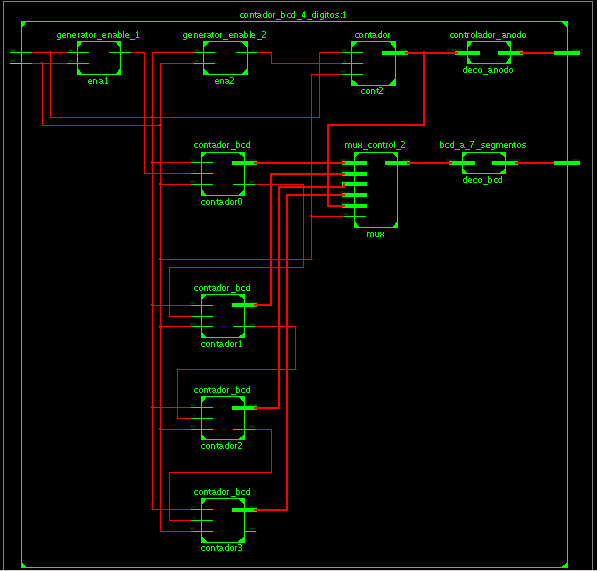
\includegraphics[scale=0.4]{./graficos/diagrama_contador_bcd_4.png}
\end{center}
\caption{Diagrama en bloque de Contador BCD de 4 dígitos}
\label{grafico1}
\end{figure}

\section*{Gráficos}
A continuación se muestran los gráficos de varias simulaciones.
\begin{figure}[h!]
\begin{center}
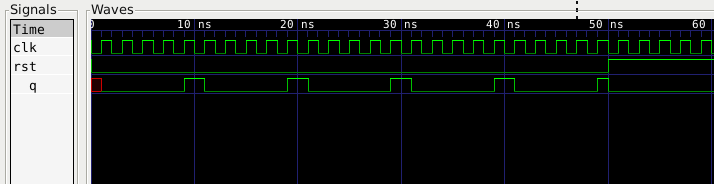
\includegraphics[scale=0.5]{./graficos/generador_enable.png}
\end{center}
\caption{Simulación de generador de enable. Genera un pulso en \textbf{q} 
	cada 5 pulsos de clock.} 
\label{grafico_enable}
\end{figure}

\begin{figure}[h!]
\begin{center}
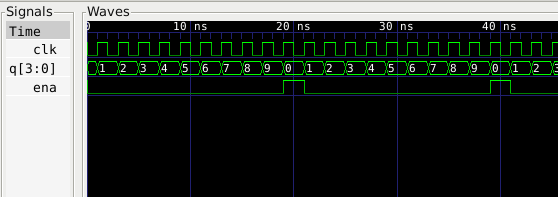
\includegraphics[scale=0.5]{./graficos/contador_bcd.png}
\end{center}
\caption{Simulación de contador BCD. Se genera un pulso de \textbf{ena} cada 
	vez que la cuenta \textbf{q} pasa de 9 a 0. }
\label{grafico_contador_bcd}
\end{figure}

\begin{figure}[h!]
\begin{center}
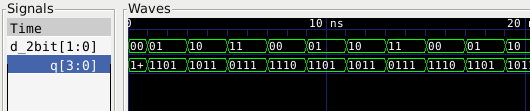
\includegraphics[scale=0.5]{./graficos/controlador_anodo.png}
\end{center}
\caption{Simulación de controlador de ánodos}
\label{grafico_controlador_anodo}
\end{figure}

\begin{figure}[h!]
\begin{center}
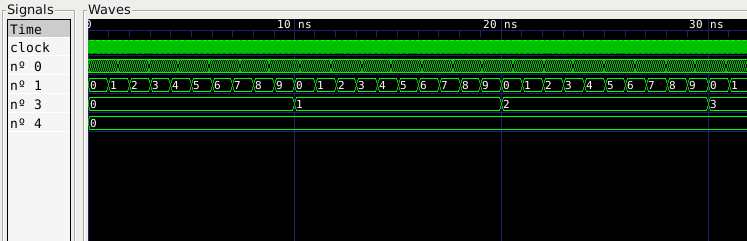
\includegraphics[scale=0.5]{./graficos/contador_bcd_4_digitos.png}
\caption{Simulación de contador BCD de 4 dígitos, incluye el clock más los 
	cuatro números}
\label{grafico_contador_4}
\end{center}
\end{figure}

\section*{Tabla de resumen de sintesis}
\begin{table}[h!]
\begin{tabular}{|c|c|c|}
\hline 
Componente & Cantidad utilizada & Porcentaje de utilización \\ 
\hline 
Slices & 134 & 2\% \\ 
\hline 
Flip-Flops & 87 & 0\% \\ 
\hline 
4 input LUTs & 252 & 2\% \\ 
\hline 
GCLKs & 1 & 4\% \\ 
\hline 
Frecuencia máxima de clock & 109.727MHz & --- \\ 
\hline 
\end{tabular} 
\end{table}

\section*{Codigo Fuente}

\subsection*{Generador de enable}
\verbatiminput{../../src/generator_enable.vhdl}

\newpage
\subsection*{Multiplexor}
\verbatiminput{../../src/mux_control_2.vhdl}

\newpage
\subsection*{Contador 2 bits}
\verbatiminput{../../src/contador.vhdl}

\newpage
\subsection*{Controlador anodo}
\verbatiminput{../../src/controlador_anodo.vhdl}

\newpage
\subsection*{Contador bcd}
\verbatiminput{../../src/contador_bcd.vhdl}

\newpage

\subsection*{Decodificador BCD a 7 segmentos}
\verbatiminput{../../src/bcd_a_7_segmentos.vhdl}

\newpage
\subsection*{Contador BCD 4 digitos}
\verbatiminput{../../contador_bcd_4_digitos.vhdl}

\end{document}
